%%
%% Copyright 2019-2021 Elsevier Ltd
%%
%% This file is part of the 'CAS Bundle'.
%% --------------------------------------
%%
%% It may be distributed under the conditions of the LaTeX Project Public
%% License, either version 1.2 of this license or (at your option) any
%% later version. The latest version of this license is in
%% http://www.latex-project.org/lppl.txt
%% and version 1.2 or later is part of all distributions of LaTeX
%% version 1999/12/01 or later.
%%
%% The list of all files belonging to the 'CAS Bundle' is
%% given in the file `manifest.txt'.
%%
%% Template article for cas-sc documentclass for
%% single column output.

\documentclass[a4paper,fleqn]{cas-sc}

% If the frontmatter runs over more than one page
% use the longmktitle option.

%\documentclass[a4paper,fleqn,longmktitle]{cas-sc}

\usepackage[numbers]{natbib}
%\usepackage[authoryear]{natbib}
%\usepackage[authoryear,longnamesfirst]{natbib}
\usepackage{graphicx}
\usepackage{multirow}
\usepackage[normalem]{ulem}
\useunder{\uline}{\ul}{}
\usepackage{lscape}
\usepackage{longtable}
\usepackage{booktabs,tabularx}
\usepackage{float}
\usepackage[section]{placeins}

%%%Author macros
\def\tsc#1{\csdef{#1}{\textsc{\lowercase{#1}}\xspace}}
\tsc{WGM}
\tsc{QE}
%%%

% Uncomment and use as if needed
%\newtheorem{theorem}{Theorem}
%\newtheorem{lemma}[theorem]{Lemma}
%\newdefinition{rmk}{Remark}
%\newproof{pf}{Proof}
%\newproof{pot}{Proof of Theorem \ref{thm}}

\begin{document}
\let\WriteBookmarks\relax
\def\floatpagepagefraction{1}
\def\textpagefraction{.001}

% Short title
\shorttitle{Hybrid DL Models For Solar Irradiance Forecasting}

% Short author
\shortauthors{A Kumar}

% Main title of the paper
\title [mode = title]{Hybrid Deep Learning Models for Solar Irradiance Forecasting of India's Cities}


\begin{comment}
% Title footnote mark
% eg: \tnotemark[1]
\tnotemark[<tnote number>]

% Title footnote 1.
% eg: \tnotetext[1]{Title footnote text}
\tnotetext[<tnote number>]{<tnote text>}

% First author
%
% Options: Use if required
% eg: \author[1,3]{Author Name}[type=editor,
% style=chinese,
% auid=000,
% bioid=1,
% prefix=Sir,
% orcid=0000-0000-0000-0000,
% facebook=<facebook id>,
% twitter=<twitter id>,
% linkedin=<linkedin id>,
% gplus=<gplus id>]

\author[<aff no>]{Amod Kumar}[<options>]

% Corresponding author indication
\cormark[<corr mark no>]

% Footnote of the first author
\fnmark[<footnote mark no>]

% Email id of the first author
\ead{amod.cse.2021@gmail.com}

% URL of the first author
\ead[url]{<URL>}

% Credit authorship
% eg: \credit{Conceptualization of this study, Methodology, Software}
\credit{<Credit authorship details>}

% Address/affiliation
\affiliation[<aff no>]{organization={},
addressline={},
city={},
% citysep={}, % Uncomment if no comma needed between city and postcode
postcode={},
state={},
country={}}

\author[<aff no>]{<author name>}[<options>]

% Footnote of the second author
\fnmark[2]

% Email ID of the second author
\ead{}

% URL of the second author
\ead[url]{}

% Credit authorship
\credit{}

% Address/affiliation
\affiliation[<aff no>]{organization={},
addressline={},
city={},
% citysep={}, % Uncomment if no comma needed between city and postcode
postcode={},
state={},
country={}}

% Corresponding author text
\cortext[1]{Corresponding author}

% Footnote text
\fntext[1]{}

% For a title note without a number/mark
%\nonumnote{}


\end{comment}



% Here goes the abstract
\begin{abstract}
Today's growing global population relies on energy to meet routine necessities and activities. Renewable energy sources, particularly solar power, have the potential to meet global energy demand while lessening the adverse effects of traditional sources on global warming. The most significant component of solar energy applications is solar radiation. On the other hand, access to solar radiation is regulated by several criteria, including prediction timeframes, weather categorisation, and assessment metrics, all of which should be carefully considered. Precision irradiation from the sun prediction is essential for power system designers and grid operators to operate solar-generating projects properly. Because sunlight is irregular and unpredictable, traditional statistical and machine learning methodologies frequently fail to provide meaningful estimations. Researchers in this field have employed deep learning models to solve the shortcomings of existing machine learning algorithms and improve prediction accuracy. It studies time series analysis as well as forecasting short-term solar irradiation. The primary objective is to develop forecasting models that hybridise DL techniques with data from various sources. The purpose is to anticipate solar irradiance at a specific location in India over 23 years (2001-2023). The power project delves archive contains data on daily solar exposure.
The proposed approach for measuring solar irradiation uses time series analysis with DL models. The dataset spans 23 years and provides daily records of sun irradiation for several places across India. The first critical step in our investigation is to normalise solar irradiance data. Based on time series explored characteristics, hybrid DL models such as CNN-RNN and GRU-BiLSTM-LSTM have been proposed compared to stand-alone DL models. CNN, RNN, BILSTM, LSTM, and GRU all increased prediction accuracy by 2.92\%, 1.54, 1.06\%, 0.7\%, 0.4557\%, and 0.21\%, respectively. This article provides fundamental principles that may be a foundation for implementing DL models. Field researchers and engineers might use these principles to enhance solar PV facility modelling and design, increasing solar energy consumption.
\end{abstract}

% Use if graphical abstract is present
%\begin{graphicalabstract}
%\includegraphics{}
%\end{graphicalabstract}

% Research highlights
% \begin{highlights}
% \item
% \item
% \item
% \end{highlights}

% Keywords
% Each keyword is separated by \sep
\begin{keywords}
\sep Solar Irradiance Prediction \sep Energy Management \sep Deep Learning\sep Photovoltaic Systems\sep Time Series Prediction

\end{keywords}
\maketitle

% Main text
\section{Introduction}
Solar cells are energy devices that convert solar energy directly into electrical energy. Solar cells will account for 10\% of total energy consumption in 2030, implying that renewable energy sources will account for 30\%. Solar cells can account for up to 30\%  of Asian nations' energy resources when combined with wind turbines, thermal power plants, hydroelectric power plants, and power grid-integrated batteries. Significant reliability and management difficulties may occur with additional renewable energy to maintain the power grid system operational in the face of changing weather conditions, allowing the power grid to preserve renewable energy output while adjusting for deviations. Solar irradiance forecasts must be tailored to specific application requirements, ranging from short-term to long-term. Solar irradiance changes, such as ramp occurrences, must be predicted in extremely short-term and short-term time frames. These frequent fluctuations affect the dependability and performance of photovoltaic solar power systems. Short-term forecasting accuracy is critical for anticipating maximum solar power ramp rates, allowing for improved oscillation management and reduction \cite{brahma2020solar}.

However, it is vital to recognise the importance of medium and long-term forecasting horizons for enhancing operating planning and actively participating in the power system. This larger perspective allows for more effective planning and decision-making in the rugged terrain of energy management. Demonstrated how forecasting day-ahead solar irradiance might improve energy savings in a commercial building microgrid. The microgrid can optimise its energy consumption, storage, and distribution strategies by correctly anticipating solar irradiance a day in advance. To accomplish good solar energy forecasting, a suitable forecasting approach must be chosen based on the application's requirements. These approaches can range from statistical models to machine learning (ML) techniques, and their selection is influenced by factors such as prediction scope, data availability, and computational resources. The advantages of solar energy prediction may be improved while possible interruptions and inefficiencies in energy systems are mitigated by customising the forecasting technique to the application's unique requirements. DL algorithms have lately found traction in the prediction of solar irradiation. These models, a subset of ML methodologies, were designed to address complicated problems requiring enormous amounts of data. DL is well-known for its capacity to automatically extract precise properties from raw data, allowing crucial patterns to be detected\cite{husein2019day}.

As the amount of input data rises, DL models perform better than other types of models of ML models. The performance of regular machine learning models was compared to DL models when the amount of input data was changed. According to the study's findings, the predicting accuracy of DL models improves as the amount of training data grows\cite{rajagukguk2020review}. Models of traditional ML, on the other hand, tend to plateau once a given amount of data has been collected. DL's capacity to tackle complex forecasting problems such as solar irradiance prediction is evidenced by their efficacy growing as input data increases. DL models, designed to evaluate Time-series data, including text, audio, video, and photography, have significantly progressed and accomplished grand. RNNs, LSTM networks, GRUs, and hybrid models such as CNN-RNN and GRU-BiLSTM-LSTM are among the architectures covered by these models. These DL architectures performed admirably in sequential data-based solar forecasting models. LSTM and CNN models outperform Artificial Neural Networks (ANNs) and Support Vector Machines (SVMs) in forecasting short-term global horizontal irradiance (GHI), according to research. Because of their intrinsic capacity to examine and interpret precise temporal patterns, these models are valuable tools for addressing the significant difficulties of solar energy forecasting\cite{zang2020short}.

\subsection{In summary, the following are the work's major contributions:}
\begin{enumerate}
\item The research study targets India's eleven highly solar-irradiant cities for forecasting model learning.
\item  Two novel hybrid DL models have been proposed and evaluated for all eleven cities and stand-alone DL models for comparison purposes. 
\item The RSME and MAPE performance measures are used for quantitative comparision to demonstrate the effectiveness of proposed models over traditional models, along with graphical interpretation of effective performance. 
\item Furthermore, statistical analysis through Friedman ranking is also done to show the advantages of the proposed models. 
\end{enumerate}

\section{Literature Review}
Forecasting solar power production is critical for understanding solar panels' short and long-term performance. Historical radiation data must be imported from sources such as PV-GIS, an abbreviation for Photovoltaic Geographical Information System, National Aeronautics and Space Administration (NASA) to evaluate the performance of a newly constructed solar plant. By measuring energy production viability over time, this calibration assists investors in determining the feasibility of Solar Power Plants (SPPs). Effectively forecasting solar electricity generation is a vital stage in SPP operations. Solar radiation, primarily a challenge of time series prediction, may be dealt with using Data-driven DL methods or regression. Early strategies employed linear regression on prior samples to estimate future values, such as the models such as autoregressive moving average (ARMA) and autoregressive integrated moving average (ARIMA). Although ARMA and ARIMA are useful for short-term forecasting, their use is limited since they rely on linear regression DL technologies, such as ANNs, created to overcome this non-linearity.\\
Cloud cover and bright, partly cloudy, or gloomy weather conditions impede solar generation forecasts. Multi-layer perceptron (MLP) models used in supervised learning meet this need. However, the performance of the MLP model may need to catch up to expectations. Cloud cover and bright, partly cloudy, or gloomy weather conditions impede solar generation forecasts. MLP models used in supervised learning meet this need. However, the performance of the MLP model may need to catch up to expectations. DL models, including RNNs, CNNs, LSTM, and GRUs, have emerged to solve this. These models have been demonstrated to be effective in a wide range of time-series forecasting applications.\\
A range of research methodologies are used in the research literature. The scientific literature may find numerous articles that anticipate sun irradiation using various methods. For instance, several research studies have used DL models, depending on historical solar irradiance data from various locations in India, such as Pokharan, Udaipur, Ajmer, Jodhpur, Bhuj, New Delhi, South Delhi, Ahmedabad, Hyderabad, and Bengaluru. These districts collect the data in CSV file\cite{kumari2021deep}. These tests have examined the performance of RNN, LSTM, GRU, CNN, and BiLSTM for day-ahead spatiotemporal forecasting of solar irradiation at various locations. Additionally, recommended methods for anticipating and optimising solar cell models based on various input variables include ANN and Fuzzy Logic (FL) approaches. Researchers have also examined ground imaging systems and nano waveguide theories to estimate solar radiation\cite{kumari2021deep}. The table below offers an overview of current DL models for predicting solar output. The table delves into the subject thoroughly, focusing on various computing approaches, error metrics, prediction horizons, and the authors behind these models. Each table row includes the proposed method, error metrics assessed, the prediction horizon considered, and a brief description of the model's approach. The picture demonstrates the multidisciplinary nature of solar power projections by combining ML approaches with meteorological data. It is a priceless resource for academics, practitioners, and hobbyists interested in the expanding breadth of applications in solar energy forecasting.

% Please add the following required packages to your document preamble:
% \usepackage{longtable}
% Note: It may be necessary to compile the document several times to get a multi-page table to line up properly
\begin{longtable}[c]{|p{0.15\textwidth}|p{0.15\textwidth}|p{0.15\textwidth}|p{0.45\textwidth}|}
\caption{Solar Power Prediction}
\label{tab:my-table}\\
\hline
\textbf{Proposed Plan} & \textbf{Criteria} & \textbf{Forecast Range} & \textbf{Explanation} \\
\hline
\endhead
Shark Shell + NN\cite{lee2018forecasting} & MAPE, RMSE, MAE & 12 h & This article employs Simulated Annealing and NN to develop a hybrid model for 12-hour solar power estimation. The proposed technique employs both optimisation and ML methodologies to improve the accuracy of solar power projections. \\ \hline
LSTM\cite{abedinia2018solar} & RMSE & 24 h & This research develops an LSTM-based DL model for forecasting solar power. The suggested model is compared to linear regression, bagged regression trees, and NN. \\ \hline
LSTM\cite{abedinia2018solar}& RMSE & 1 min &This study provides an LSTM-based DL model for forecasting solar power. The model is compared to MLP and CNN-based models using past solar radiation and sky photos as input vectors. \\ \hline
CNN+LSTM\cite{lee2018forecasting} & RMSE, MAE, MAPE & 200 days &This work provides a CNN-LSTM hybrid DL model for a 200-day solar power forecast, and the suggested model is compared against conventional, LSTM, and additional LSTM variants. \\
CNN\cite{zhang2018deep} & RMSE & 5 min & The authors propose a CNN-based approach for predicting solar power. The cloud images are sent into the proposed CNN model as an input feature vector to train it. \\ \hline
CNN, LSTM\cite{wang2019comparison} & MAPE, RMSE, MAE & 24 h & The authors presented and evaluated three DL prediction models with varying training data. According to the study, the hybrid model outperforms other models in prediction. \\ \hline
LSTM\cite{lee2019deep} & RMSE & 19 h & This study provides a Solar DL model based on LSTM for solar power forecasting. The model is evaluated in comparison to ARIMA and NN-based models. \\
Feed Forward NN\cite{torres2019big} & RMSE, MAE & 24 h & The solar power forecast approach employs massive H2O and Apache Spark data time series analysis package. The proposed model was trained using two years of Australian solar data. \\ \hline
RNN+LSTM\cite{hu2021short} & RMSE, MAE & 24 h &Based on RNN+ LSTM, this study presents a DL model for anticipating short-term solar power. Data from the solar power plant is used as the input vector. The proposed model is compared against deep learning models based on RNN, LSTM, and DNN. \\\hline
LSTM\cite{husein2019day} & RMSE, MAE, Forecast skill & 24 h &The author developed and compared an LSTM-based DL model for forecasting short-term solar irradiance to feed-forward NN (FFNN). The United States, Germany, Switzerland, and South Korea offer input data. By a factor of two, the suggested model outperforms FFNN. \\ \hline
CNN+LSTM\cite{de2019solar} &RMSE, MAE, MAPE & 1,3 days & A CNN-LSTM hybrid DL model is presented in this study. The suggested model is compared to LSTM, RNN, which is CNN, and GRU-based DL methods one and three days ahead of the renewable energy forecast. \\ \hline
Wavelet Decomposition (WPD) +LSTM\cite{li2020hybrid} &MAPE, RMSE, MAE & 300 mins &This paper provides a WPD+ LSTM-based predictions of short-term solar power using the DL model. DL models based on LSTM, GRU, BILSTM, CNN, and RNN outperform the suggested hybrid model. \\ \hline
RNN\cite{cao2005forecast} &RMSE & 1 Day (hourly) & solar irradiance 1990-2022( 12107 days) \\ \hline
RNN\cite{niu2017recurrent} & RMSE & 10 minutes, 30 minutes, 1 hour & solar radiation temperature of the dry bulb and relative humidity The degree of humidity from May 22 to May 29, 2016 (7 days). \\ \hline
LSTM\cite{qing2018hourly} & RMSE & 1 Day ahead &temperature, relative humidity, visibility, and wind speed (March-August 2012, January-December 2013). \\ \hline
CNN-LSTM, LSTM\cite{wang2018wavelet} & RMSE & Every 15 Min & solar irradiance from 2008 to 2011, and again from 2014 to 2017 (3013 days) \\
\hline
\end{longtable}


\section{Data Processing}

\subsection{Enclosed Region and Target Area}
Figure \ref{Figure 1}Latitude and longitude are geographic coordinates used to determine exact places on the Earth's surface. They are measured in degrees, with latitude representing north-south and longitude representing east-west. There are three key benefits of collecting latitude and longitude data for Indian cities as Bhuj(23.2531, 69.6693), Pokhran(27.0953, 71.7566), Jodhpur(26.2389, 73.0243), Udaipur(24.5854, 73.7175), Bengaluru(12.9716, 77.5946), Hyderabad(17.3850, 78.4867), Ahmedabad(23.0338, 72.5850), Ahmedabad2(23.0225, 72.5714), New Delhi(28.6139, 77.2090), South Delhi(28.4852, 77.1964), Ajmer(26.4499, 74.6399). The investigation focuses on a single target point many sites surrounding the target region within the limited zone. Data gathering at the specified location, a near-real-time 0.455 × 0.625-degree data set is obtained for the data from the target point. The destination location's decimal degree longitude and latitude are specified in a numeric vector format to generate this data collection. For the regional coverage, lat/log region = 381.65 meters degrees of 0.455 × 0.625 degrees. In the case study for solar irradiance forecast, a numerical vector of length eleven was used to represent the contained region. This vector contains latitude and longitude coordinates for the lower-left and upper-right corners of the enclosing box. The lower-left corner has five coordinates, and the upper-right corner has five coordinates, plus one extra value, in an 11-data vector \cite{belmahdi2020one}.

\subsection{Data Collection}
Due to a lack of ground-based temperature, it claims to have utilised historical time series and satellite data from NASA's POWER database. The data set spans 23 years, from 2001 to 2023, and consists of daily observations of solar irradiance in kilowatt-hours per square meter. This text accurately describes the data source utilised in the study; hence, it does not appear to be plagiarised. If you use this material in your work, remember to properly cite the source to give credit to the researchers who gathered and made the data available. Academic honesty and appreciating the contributions of others to research need proper citation. The forecasting challenge aims to predict solar irradiance data for a target location. Conversely, the model incorporates data from the surrounding region rather than just the target location. This strategy attempts to reduce data dependency on extraneous qualities while correcting data flaws in the target location.
High Solar Irradiance cities data was collected from eleven cities in India: Udaipur, Ajmer, Jodhpur, Pokharan, Bhuj, Hyderabad, Ahmedabad, South Delhi, New Delhi, and Bengaluru. The NASA POWER regional data access widget gave the forecasting data, which provides data access in near-real time. The objective area as well as the data region for solar irradiance. The data collecting and processing methods utilised in a case study The offered information describes methods for predicting solar irradiation. The important points are summarised here\cite{brahma2020solar}.

\begin{itemize}
\item
Deep learning models for calculating daily solar irradiation were designed and deployed as part of the research. These models were built to forecast correctly using historical data.
\item
The models were created and verified using univariate and multivariate solar irradiance data from a single location. This allowed for a comparison of the model's performance under different settings.

\item
Traditional performance evaluation measures were utilised to examine the developed models' accuracy, performance, and dependability. A rolling window assessment technique was utilised to analyse how well the models performed over time.
\item
The research examined how surrounding region characteristics affected solar irradiance forecasts for the target regions. NASA solar irradiance data gathered over 23 years was used in this investigation.

\end{itemize}

\subsection{Data Preprocessing}
Identify and manage missing values in the dataset, including imputation and row or column removal. Find and eliminate duplicate records in the dataset. Outliers are data points that differ significantly from the average and must be discovered and addressed.EDA is used to discover patterns and trends in data distribution and variable interactions. Maintain a record of all pretreatment processes and data changes. Replication requires this documentation. Examine the preprocessed data to verify if it was appropriately prepared for use as input for machine learning or deep learning models. This might include changing data or creating sequences for time series models.
\begin{itemize}
\item
Data Input: In this step, download data from NASA's website in the CSV file format; multivariate data was downloaded in Indian cities' high solar irradiant areas. The downloaded dataset is used as program input.

\item
Data Preprocessing: In this step, missing values are imputed by means. Each data work 30 iteration and 200 epochs and take the mean of all dataset.
After missing value imputing on the dataset, use min-max scaling by min-max scaling features to scale in the range [0,1].
\begin{equation}
y_{dc}=\frac{y-min(y)}{max(y)-min(y)}
\end{equation}
Here, y is the original value of a cell, min(y) is the minimum value of the column, and max(y) is the maximum value of the column.
\end{itemize}


\begin{figure}[!ht]
\centering
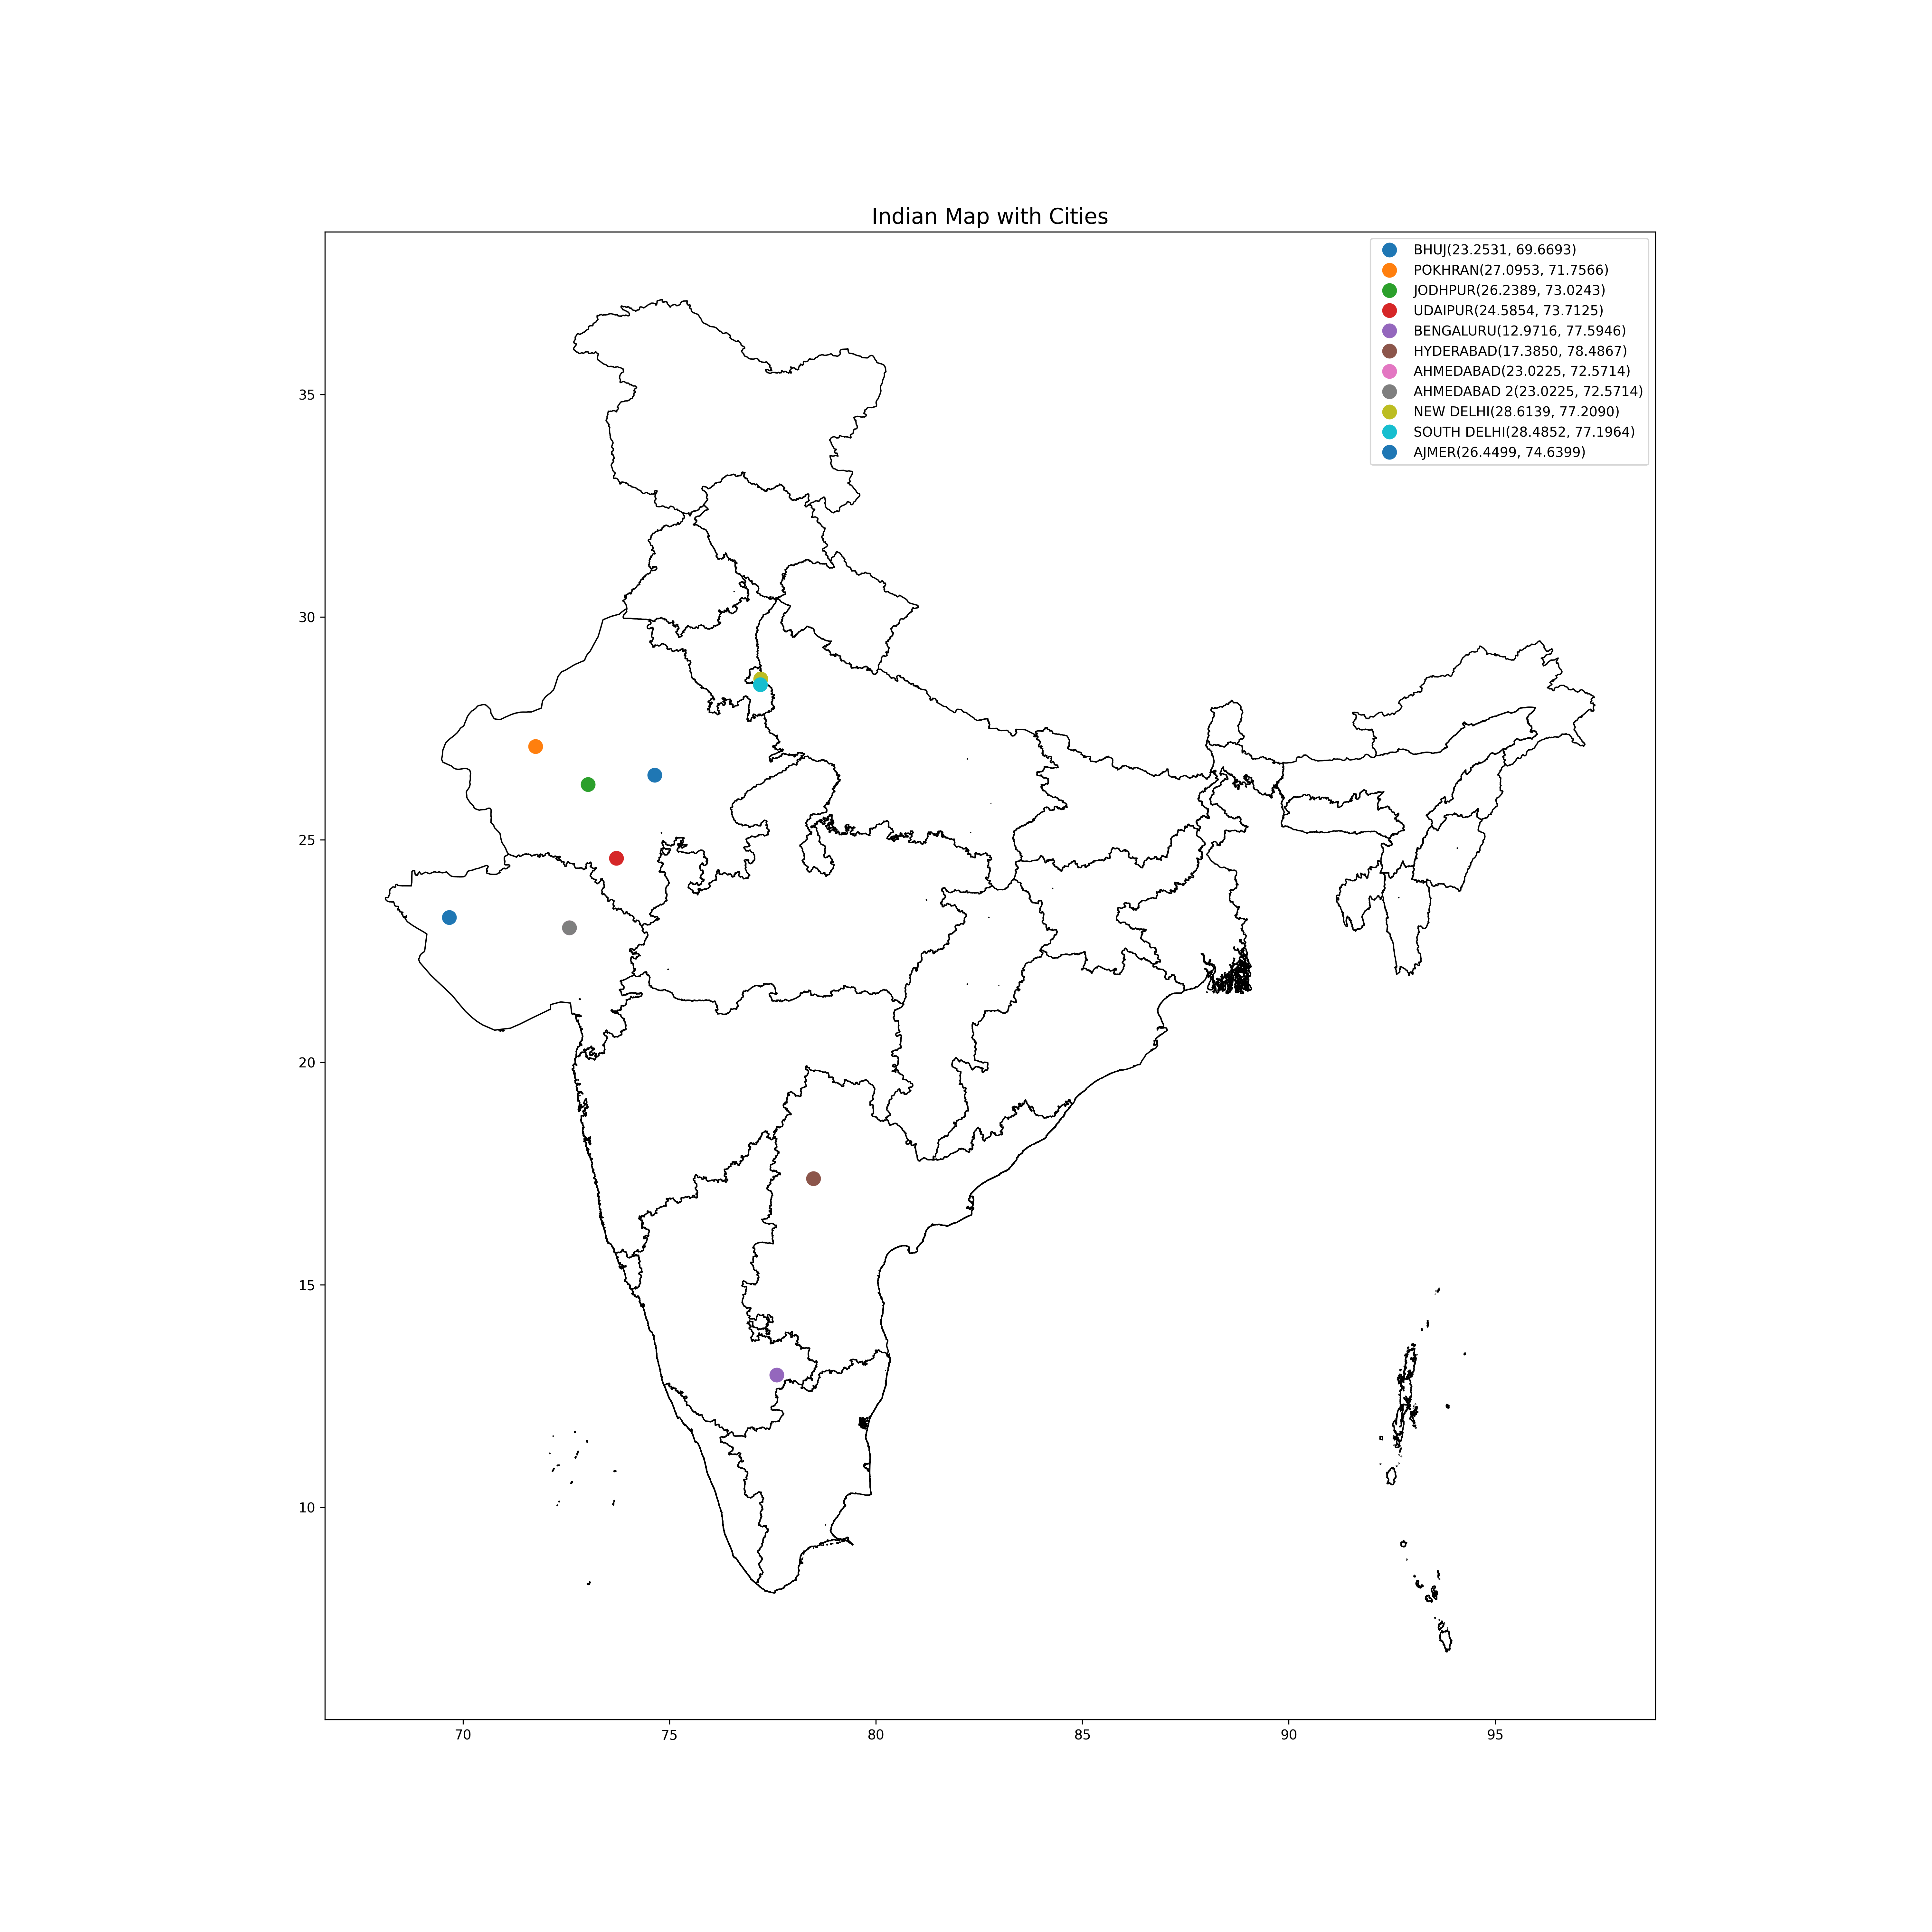
\includegraphics[width=\textwidth]{AMod India_Map}
\caption{Data location with latitude and longitude of the eleven cities of India }
\label{Figure 1}
\end{figure}



\section{Deep Learning Models}
The DL models are composed of several neural networks tuned for specific tasks. CNNs are particularly adept in image processing and feature extraction. LSTM networks manage long-range relationships within sequences, whereas RNNs specialise in sequential data processing. GRUs are a more straightforward alternative to LSTMs. Unsupervised feature learning is performed using Deep Belief Networks (DBNs). Data is compressed into a lower-dimensional space via autoencoders. GANs (Generative Adversarial Networks) produce realistic data samples. Transformers with self-attention mechanisms are transforming natural language processing. Each model is essential in various applications, boosting computer vision, language understanding, and natural language processing.

\subsection{CNN:} The language you supplied describes the convolutional layer, a fundamental component of a CNN. The following section briefly discusses the sentence's subjects. CNN is a deep neural network architecture that recognises images\cite{hao2018optimized,chauhan2018convolutional} and videos\cite{fan2016video,he2021automatic,qi2018cnn}. Its popularity has soared thanks to its ability to learn and extract critical information from photographs automatically. The three basic types of layers are convolutional, pooling, and fully connected, which form the typical CNN architecture. Stacking these levels on top of one another allows for extracting characteristics from a hierarchy\cite{torres2021deep}.

1. Convolutional Layer:
\begin{equation}
\mathbf{Z} = \mathbf{D} * \mathbf{X} + \mathbf{b}
\end{equation}

2. Activation Function:
\begin{equation}
\mathbf{A} = \sigma(\mathbf{Z})
\end{equation}

3. Layer of Collection:
\begin{equation}
\mathbf{P} = \text{Collection}(\mathbf{A})
\end{equation}

4. Fully Connected Layer:
\begin{equation}
\mathbf{O} = \mathbf{D}_\text{fc} \cdot \mathbf{P} + \mathbf{b}_\text{fc}
\end{equation}

Here, $\mathbf{D}$ represents the convolutional filter weights, $\mathbf{X}$ is the input data, $\mathbf{b}$ is the bias term, $\sigma$ is the activation function (e.g., ReLU), $\mathbf{A}$ is the activation map, $\text{pool}$ denotes pooling operation (e.g., max pooling), $\mathbf{P}$ is the pooled output, $\mathbf{D}_\text{fc}$ is the weight matrix for the fully connected layer, $\mathbf{b}_\text{fc}$ is the bias term for the fully connected layer, and $\mathbf{O}$ is the final output.











\subsection{RNN}
GRU was proposed as an RNN. It was designed to be a less formal and complex alternative to more sophisticated. While still processing sequential data such as text, audio, and time series data, LSTM networks are used. GRU works by introducing gating mechanisms that allow for specific modifications to the network. At each time step, a concealed state is revealed. These gating techniques are crucial for regulating data flow across the network. Unlike traditional RNNs, GRU has two fundamental gating mechanisms: reset gate and update gate\cite{sun2016depth}. A neural network's reset gate determines how much of the prior hidden state should be forgotten or reset for the current calculation, allowing the model to manage the preservation or omission of information from earlier time steps or layers. This gate enables the model to retain essential previous data while eliminating less critical data. The update gate, on the other hand, specifies how much the incoming input should contribute to updating the concealed state. GRU can identify the significance of incoming input in the context of the present state by managing the updating process\cite{torres2021deep}.




1. Hidden State Update:
\begin{equation}
h_c = \tanh(D_{hh} \cdot h_{c-1} + D_{xh} \cdot x_c)
\end{equation}

2. Output Calculation:
\begin{equation}
y_c = D_{hy} \cdot h_c
\end{equation}
The hyperbolic tangent activation function is represented by the symbol $tanh$, In an RNN or similar architectures, $D_{hh}$ is a weight matrix used to change the previous hidden state ($h_{c-1}$),$D_{xh}$ is a weight matrix that is applied to the input at time step $c$ ($x_c$) before it is used to calculate the new hidden state ($h_c$),$D_{hy}$ is a weight matrix that is used to turn the hidden state ($h_c$) into the output ($y_c$) at a specific time step, The concealed state from the previous time step is denoted by $h_{c-1}$.




% Reset Gate (r):
% \begin{equation}
% 𝑟𝑡 = 𝑠𝑖𝑔𝑚𝑜𝑖𝑑(𝑊𝑟 * [ℎ(𝑡 − 1), 𝑥(𝑡)] + 𝑏𝑟)
% \end{equation}

% Update Gate (z):
% \begin{equation}
% 𝑧(𝑡) = \𝑠𝑖𝑔𝑚𝑜𝑖𝑑(𝑊𝑧 ∗ [ℎ(𝑡 − 1), 𝑥(𝑡)] + 𝑏𝑧)
% \end{equation}

% Candidate Hidden State ( h):
% \begin{equation}
% ℎ(𝑡) = 𝑡𝑎𝑛ℎ(𝑊ℎ ∗ [𝑟(𝑡) ℎ(𝑡 − 1), 𝑥(𝑡)] + 𝑏ℎ)
% \end{equation}

% Updated Hidden State (h):
% \begin{equation}
% ℎ(𝑡) = (1 − 𝑧(𝑡)) ℎ(𝑡 − 1) + 𝑧(𝑡)ℎ(𝑡)
% \end{equation}



\subsection{GRU}
The GRU represents a significant step forward in the study of recurrent neural networks, having evolved in 2014 as a consequence of the joint efforts of the GRU, which was developed as a less sophisticated alternative to the more complex Networks with LSTM, excels in understanding data in consecutive order such as text, audio, and time series. GRU is cleverly designed around gating mechanisms, which are utilised to fine-tune the network's hidden state evolution throughout each progressive time step. These gating devices, which serve as alarm sentinels, monitor data flow in and out effectively\cite{he2019wind}. The two most critical gating components in the GRU, the reset gate and the update gate, are components of architecture\cite{wu2016investigating,khadka2017evolving}. GRU has been carefully designed around gating mechanisms, which are utilised to perfectly fine-tune the network's hidden state growth as each progressive time step advances. These gating devices, which serve as alarm sentinels, effectively monitor data flow in and out. The two most critical gating components in the GRU's architecture are the reset gate and the update gate\cite{badescu2008modeling}. GRU's operation is mathematically characterised as follows:


1. Update Gate ($z_c$):
\begin{equation}
p_c = \sigma(D_z \cdot [h_{c-1}, x_c])
\end{equation}

2. Reset Gate ($r_c$):
\begin{equation}
r_c = \sigma(D_r \cdot [h_{c-1}, x_c])
\end{equation}

3. Candidate Memory ($\tilde{h}_c$):
\begin{equation}
\tilde{h}_c = \tanh(D_h \cdot [r_c \odot h_{c-1}, x_c])
\end{equation}

4. Hidden State Update ($h_c$):
\begin{equation}
h_c = (1 - z_c) \odot h_{c-1} + z_c \odot \tilde{h}_c
\end{equation}

Here, $\sigma$ represents the sigmoid activation function, $\odot$ denotes element-wise multiplication, and $D_z$, $D_r$, and $D_h$ are weight matrices learned during training. $x_c$is the time step input $c$, $h_{c-1}$is the previous concealed state, and $h_c$ is the new hidden state.





\subsection{LSTM}
LSTM network is a significant improvement in RNNs, mainly created to overcome problems faced by prior RNNs. Traditional RNNs need to improve in maintaining information over lengthy periods. These networks fail to maintain a memory trail through significant temporal gaps, making them unfit for complex tasks requiring the capture of "long-term dependencies." Such dependencies necessitate the long-term retention of contextual information, which regular RNNs are incapable of. In contrast, LSTM networks have much promise for reducing these gaps. Memory cells capable of storing information for extended periods are at the heart of their distinct design\cite{abdel2020reliable}. This deliberate inclusion allows LSTMs to carefully preserve and remember essential information from the distant past, allowing precise prediction of current occurrences. LSTMs distinguish themselves by providing unrivalled control over how much prior knowledge is retained and how much specific context components are considered redundant. Because memory preservation and pruning are entirely synced, LSTMs may be able to fine-tune the relevance of previous data, enhancing their ability to discover crucial patterns and correlations that lead to correct predictions\cite{shireen2018iterative}.



1. Forget about Gate:
\begin{equation}
f_c = \sigma(D_f \cdot [h_{c-1}, x_c] + b_f)
\end{equation}

2. Input Gate:
\begin{equation}
i_c = \sigma(D_i \cdot [h_{c-1}, x_c] + b_i)
\end{equation}

3. Candidate Memory:
\begin{equation}
\tilde{C}_c = \tanh(D_C \cdot [h_{c-1}, x_c] + b_C)
\end{equation}

4. Update Memory:
\begin{equation}
C_c = f_c \odot C_{c-1} + i_c \odot \tilde{C}_c
\end{equation}

5. Gate of Output:
\begin{equation}
o_c = \sigma(D_o \cdot [h_{c-1}, x_c] + b_o)
\end{equation}

6. Hidden State:
\begin{equation}
h_c = o_c \odot \tanh(C_c)
\end{equation}

The sigmoid activation function is represented by $sigma$, the hyperbolic tangent activation function is represented by $tanh$, and the weight matrices are represented by $D_f$, $D_i$, $D_C$, and $D_o$. Bias words include $b_f$, $b_i$, $b_C$, and $b_o$. $x_c$ represents the input at time step $c$, $h_{c-1}$ represents the previous hidden state, and $f_c$, $i_c$, $tilde{C}_c$, $C_c$, $o_c$, and $h_c$ represent the forget gate, input gate, candidate memory, updated memory, output gate, and hidden state.







\subsection{BiLSTM}
BiLSTM is a critical technique in this field. BiLSTMs are a kind of LSTM that have been demonstrated to increase model performance in sequence classification tasks. BiLSTMs make use of the bidirectional information flow of a sequence. In contrast to typical LSTMs, which analyse data sequentially in one direction, BiLSTMs employ two parallel LSTM layers. The first LSTM processes the whole input sequence, while the second LSTM reverses it. Due to its one-of-a-kind architecture, the model can collect Contextual information from the past and future for each item in the sequence. As a result, it gives a more comprehensive understanding of the sequence, leading to improved performance in tasks like emotion classification\cite{heidari2020short,rajabi2020multi,joshi2022deep}. One of the most essential characteristics of BiLSTMs is their ability to capture sequence dependencies in both directions. Contextual signals can appear before and after a particular word or phrase, which is valuable for occupations requiring text data. By considering these bidirectional connections, BiLSTMs increase the model's ability to identify complex patterns and nuances in text, resulting in more accurate emotion predictions. Bidirectional processing also increases the model's efficiency. The model may give more context without significantly increasing processing time by evaluating the inverted sequence alongside the original sequence. This dual-processing strategy both accelerates training and assists the model in making more accurate predictions\cite{wang2011solar}.



1. Forward LSTM Equations:
(Forget Gate)
\begin{equation}
f_c^{\text{F}} = \sigma(D_f^{\text{F}} \cdot [h_{c-1}^{\text{F}}, x_c] + b_f^{\text{F}})
\end{equation}

Input Gate:
\begin{equation}
i_c^{\text{F}} = \sigma(D_i^{\text{F}} \cdot [h_{c-1}^{\text{F}}, x_c] + b_i^{\text{F}})
\end{equation}

Candidate Memory:
\begin{equation}
\tilde{C}_c^{\text{F}} = \tanh(D_C^{\text{F}} \cdot [h_{c-1}^{\text{F}}, x_c] + b_C^{\text{F}})
\end{equation}

Update Memory:
\begin{equation}
C_c^{\text{F}} = f_c^{\text{F}} \odot C_{c-1}^{\text{F}} + i_c^{\text{F}} \odot \tilde{C}_c^{\text{F}}
\end{equation}

Output Gate:
\begin{equation}
o_c^{\text{F}} = \sigma(D_o^{\text{F}} \cdot [h_{c-1}^{\text{F}}, x_c] + b_o^{\text{F}})
\end{equation}

Hidden State:
\begin{equation}
h_c^{\text{F}} = o_c^{\text{F}} \odot \tanh(C_c^{\text{F}})
\end{equation}

2. Backward LSTM Equations:
(Similar to forwarding LSTM Equations, but using separate weights and biases)

3. BiLSTM Output:
\begin{equation}
h_c^{\text{B}} = [h_c^{\text{F}}, h_c^{\text{B}}]
\end{equation}

Here, $\sigma$ represents the sigmoid activation function, $\tanh$ is the hyperbolic tangent activation function, $D$ and $b$ are weight matrices and bias terms respectively, $x_c$ is the input at time step $c$, $h_{c-1}$ is the previous hidden state, $f_c$, $i_c$, $\tilde{C}_c$, $C_c$, $o_c$, and $h_c$are the forget gate, the input gate, the candidate memory, the updated memory, the output gate, and the hidden state, in that order. The superscripts "F" and "B" designate the orientations of the Forward and BiLSTM, respectively, and $h_c\text{ B}$ is the Bidirectional LSTM's final output.





\section{Model Implementation and Evaluation}

We have proposed two hybrid models, CNN-RNN and GRU-BILSTM-LSTM, which are stand-alone where the descriptions are as follows:

\subsection{Proposed1(CNN-RNN)}A 1D Convolutional layer with 32 filters and a kernel size of 3 is added. The ReLU's activation function is employed. The input shape determines the length and number of features in the sequences. A MaxPooling layer with a pool size of 2 is added. As a result, the dimensionality of the feature maps is decreased. Another Conv1D layer is added this time with 64 filters and kernel size 3. ReLU activation is used.
Another MaxPooling layer with pool size two is added.\\
\textbf{Model Compilation:} The model is built using the Adam optimiser and the MAE loss function. The model summary function generates a summary of the model's architecture, including the layer types, output shapes, and total number of parameters shown in Figure 2. This architecture combines the capabilities of CNNs (for feature extraction) with RNNs (for sequence modelling) to address applications that need sequential data. The CNN layers are responsible for learning hierarchical features, whereas the LSTM layer is responsible for acquiring sequential patterns. The model's performance is affected by the subject and dataset to which it is applied. More fine-tuning and testing may be necessary for the best results.




\begin{figure}[!ht]
\centering
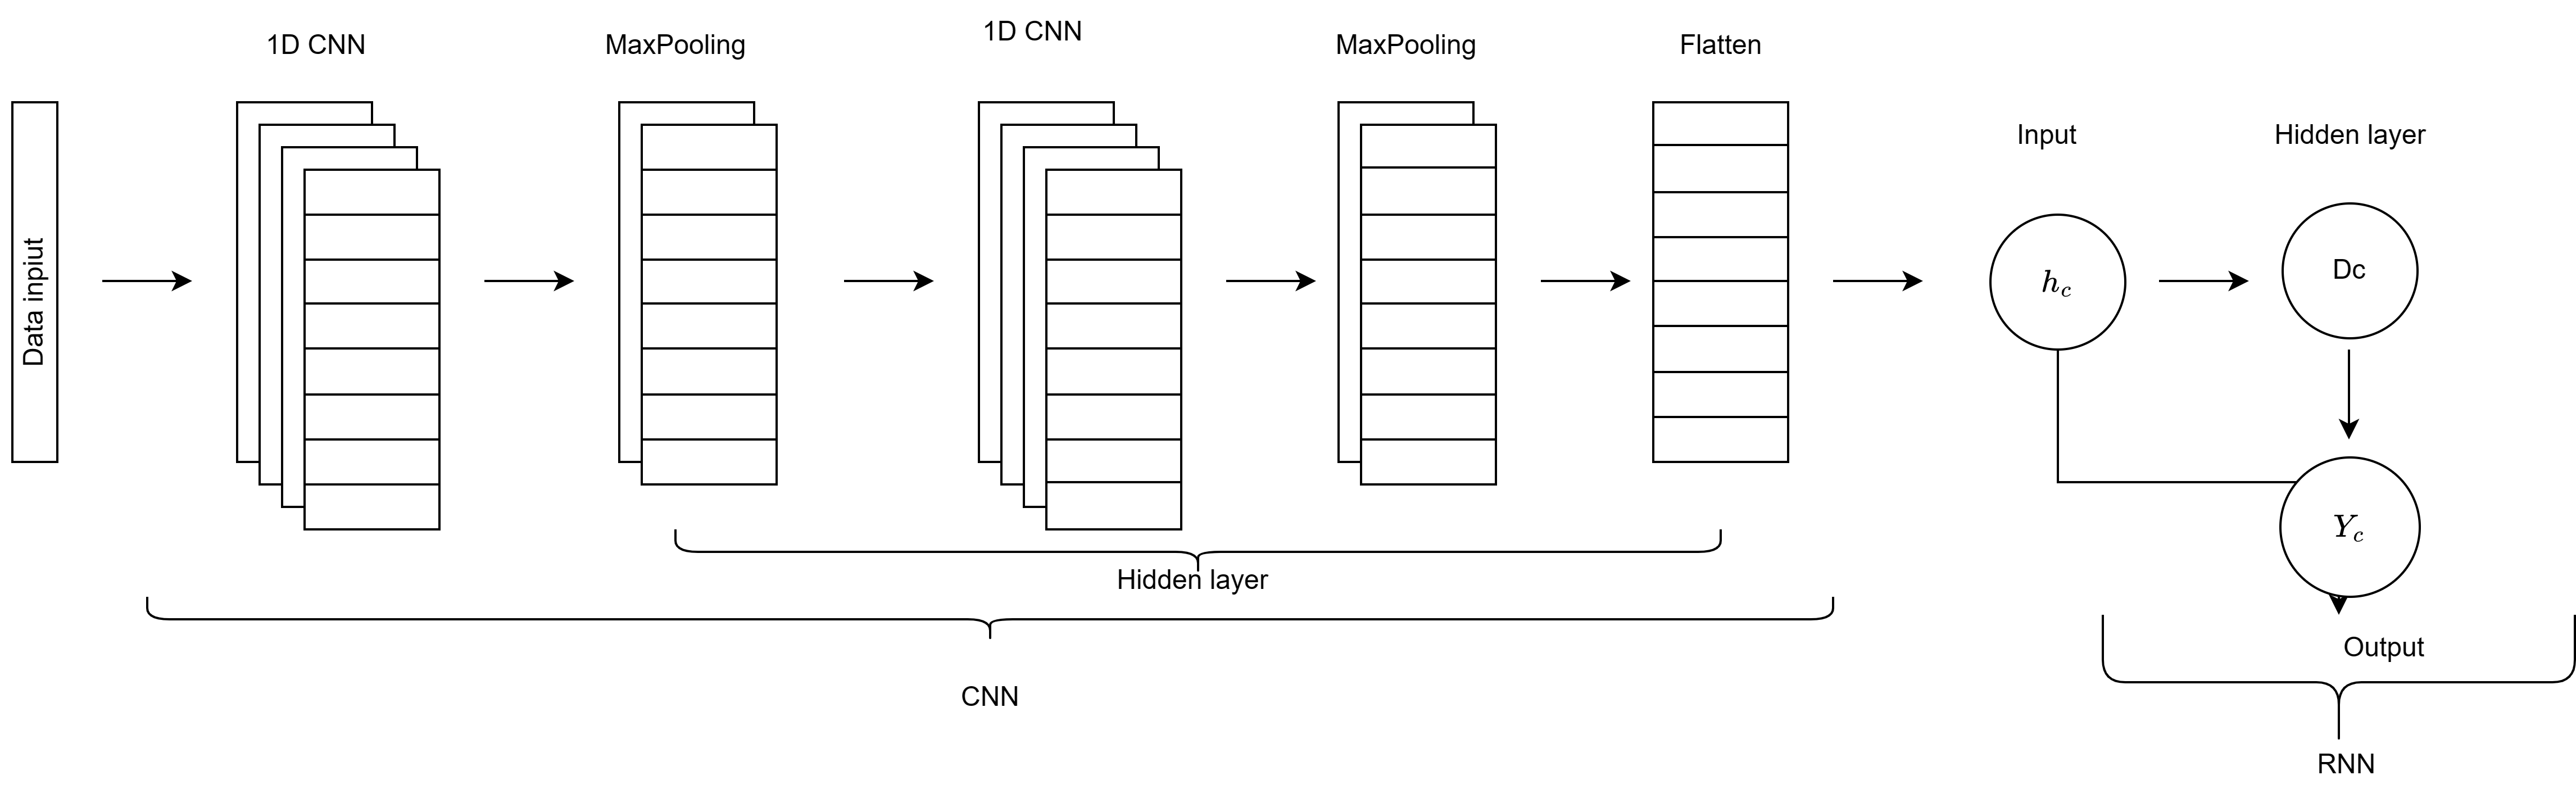
\includegraphics[width=\textwidth]{CNN-RNN (1)}
\caption{Architecture of Proposed1(CNN-RNN)}
\label{}
\end{figure}





1. Convolutional Layer:
\begin{equation}
\mathbf{Z}_{\text{conv}} = \mathbf{D}_{\text{conv}} * \mathbf{X} + \mathbf{b}_{\text{conv}}
\end{equation}

2. Activation Function for Convolutional Layer:
\begin{equation}
\mathbf{A}_{\text{conv}} = \sigma(\mathbf{Z}_{\text{conv}})
\end{equation}

3. Reshape for RNN Input:
\begin{equation}
\mathbf{X}_{\text{rnn}} = \text{reshape}(\mathbf{A}_{\text{conv}})
\end{equation}

4. RNN Hidden State Update:
\begin{equation}
\mathbf{h}_c = \tanh(\mathbf{D}_{\text{rnn}} \cdot \mathbf{h}_{c-1} + \mathbf{D}_{\text{xrnn}} \cdot \mathbf{x}_c + \mathbf{b}_{\text{rnn}})
\end{equation}

5. RNN Output Calculation:
\begin{equation}
\mathbf{Y}_c = \mathbf{D}_{\text{out}} \cdot \mathbf{h}_c + \mathbf{b}_{\text{out}}
\end{equation}

In this case, the convolutional filter weights are represented by $\mathbf{D}_\text{conv}$. The input data is represented by $\mathbf{X}$. The bias term for the convolutional layer is $\mathbf{b}_\text{conv}$, while the activation function (e.g., ReLU) for the convolutional layer is $sigma$. The activation map from the convolutional layer is $\mathbf{A}_\text{conv}$. $\text{reshape}$ is used to reshape the activation map for RNN input. The weight matrix for the RNN hidden state update is $\mathbf{D}_\text{rnn}$, the weight matrix for the RNN input is $\mathbf{b}_\text{rnn}$, and the bias term for the RNN is $\mathbf{b}_\text{rnn}$. $\mathbf{h}_c$ represents the RNN hidden state at time step $c$, $\mathbf{x}_c$ represents the input at time step $c$, $\mathbf{D}_\text{out}$ represents the weight matrix for the RNN output computation, $\mathbf{b}_\text{out}$ represents the bias term for the RNN output, and $\mathbf{Y}_c$ represents the output at time step $c$.



\subsection{Proposed2(GRU-BILSTM-LSTM)}
\textbf{layer1:}A GRU layer with the requisite number of units is added. It is set to return sequences (return-sequences=True) and requires shape data as input.
A BiLSTM layer is used. This layer explores sequences both forward and backwards, providing more background information.\\
\textbf{layer2:} An extra LSTM layer is added. It, like the first GRU layer, returns sequences. A dropout layer is used to prevent overfitting. It encourages regularisation by randomly changing during training; some input units are set to zero updates. Another GRU layer is added that does not return sequences.
Another dropout layer follows the second GRU layer. A connected thick layer of 1 unit is applied to the final product. It gives back a single scalar forecast.

\textbf{Model Compilation:}The Adam optimiser, an adaptive learning rate optimisation technique, is used to build the model. The loss function used is MAE, which determines the absolute difference between expected and actual data. To conclude, this model employs regularisation dropout and recurrent layers GRU, Bidirectional LSTM, and LSTM. The objective is to create a complex architecture that recognises temporal patterns in sequential data. The MAE loss is used for training, and the model is designed to generate a single prediction for the given input sequence.



\begin{figure}[!ht]
\centering
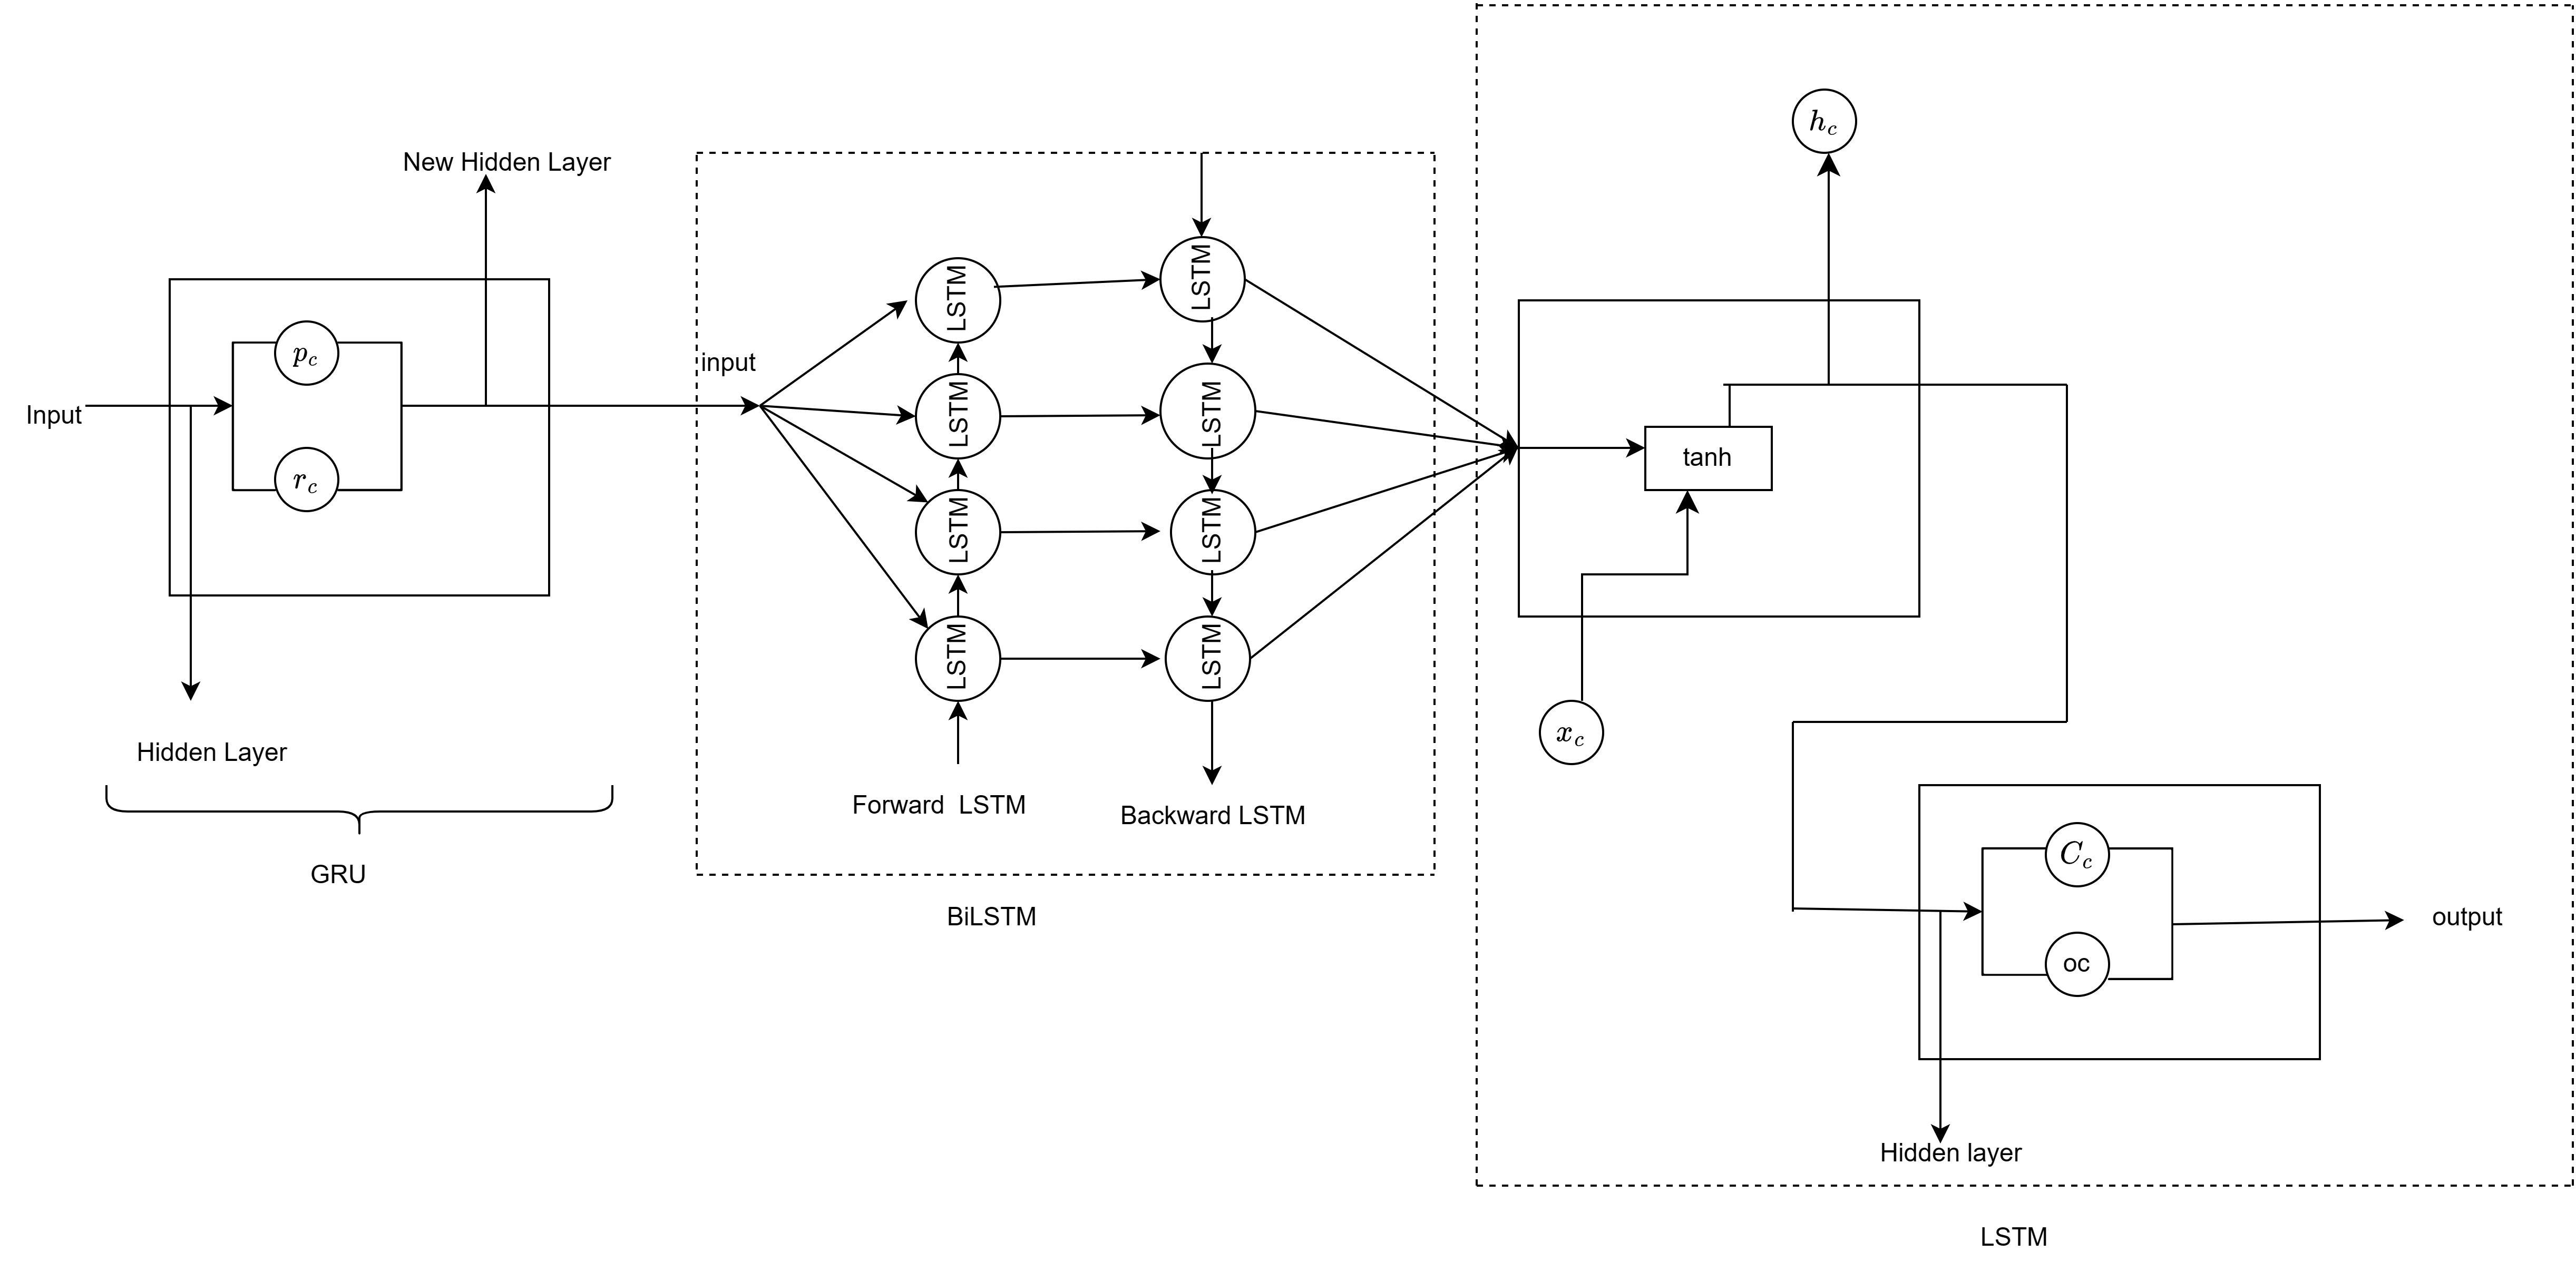
\includegraphics[width=\textwidth]{GRU-BiLSTM-LSTM (1)}
\caption{Architecture of Proposed2(GRU-BiLSTM-LSTM)}
\label{}
\end{figure}




1. GRU Equations:
(Update Gate$z_c$):
\begin{equation}
p_c = \sigma(D_z \cdot [h_{c-1}, x_c])
\end{equation}

Reset Gate ($r_c$):
\begin{equation}
r_c = \sigma(D_r \cdot [h_{c-1}, x_c])
\end{equation}

Candidate Memory ($\tilde{h}_c$):
\begin{equation}
\tilde{h}_c = \tanh(D_h \cdot [r_c \odot h_{c-1}, x_c])
\end{equation}

Hidden State Update ($h_c$):
\begin{equation}
h_c = (1 - z_c) \odot h_{c-1} + z_c \odot \tilde{h}_c
\end{equation}

2. Bidirectional LSTM Equations:
Forward(F) LSTM:
(Similar to LSTM equations)

Backward(B) LSTM:
(Similar to LSTM equations)

3. LSTM Equations:
Forget Gate:
\begin{equation}
f_c = \sigma(D_f \cdot [h_{c-1}, x_c] + b_f)
\end{equation}

Input Gate:
\begin{equation}
i_c = \sigma(D_i \cdot [h_{c-1}, x_c] + b_i)
\end{equation}

Candidate Memory:
\begin{equation}
\tilde{C}_c = \tanh(D_C \cdot [h_{c-1}, x_c] + b_C)
\end{equation}

Update Memory:
\begin{equation}
C_c = f_c \odot C_{c-1} + i_c \odot \tilde{C}_c
\end{equation}

Output Gate:
\begin{equation}
o_c = \sigma(D_o \cdot [h_{c-1}, x_c] + b_o)
\end{equation}

Hidden State:
\begin{equation}
h_c = o_c \odot \tanh(C_c)
\end{equation}

The sigmoid activation function is represented by $\sigma$, the hyperbolic tangent activation function is represented by $tanh$, the weight matrices and bias terms are represented by $D$ and $b$, the input at time step $c$ is represented by $x_c$, and the prior hidden state is represented by $h_{c-1}$, $z_c$, $r_c$, $\tilde{h}_c$, $h_c$ are the GRU update gate, reset gate, candidate memory, and hidden state respectively. The Bidirectional LSTM equations are similar to regular LSTM equations, and the LSTM equations are standard. The model combines these three recurrent layer types to process sequential data.



\begin{table}[!ht]
\centering
\caption{Values of Parameter of Models}
%\label{Algorithm Parameters-table}
\begin{tabular}{|p{0.4 \textwidth}| p{0.4 \textwidth}|}
\hline
Algorithm Parameters & Values \\ \hline
filter & 32 \\
kernel sise & 3 \\
MaxPooling & 2 \\
Activation & ReLU \\
Optimizer & Adam \\
Loss Function & MSE \\ \hline
\label{Table 2}
\end{tabular}
\end{table}


\subsection{Experimental Setup} The most critical algorithm parameters and their values are shown in the table below. The "Filter Count" option is set to 32, indicating the number of filters or convolutional units used in a convolutional layer. The option "Kernel Size" is set to 3, indicating that the convolutional kernel used in feature extraction has a size of 3. The "MaxPooling" option is set to 2, indicating that a MaxPooling operation with a pool size 2x2 is being used. The "ReLU" (Rectified Linear Unit) function is utilised for the activation function, a common choice in neural networks to generate non-linearity. The "Adam" optimiser is used during training to update the network's weights, and the "Mean Squared Error" (MSE) is utilised as the loss function to compare the model's prediction accuracy against actual values shown in Table \ref{Table 2}.

\subsection{Mean Absolute Error(MAE)}
It is calculated by averaging the absolute difference between actual and forecast solar irradiance levels throughout the whole array and dividing the result by the total number of observations in the array to obtain the mean absolute error (MAE)\cite{kumari2021deep}.

\begin{equation}
MAE = \frac{\sum_{n}^{i=1}|y_i-x_i|}{n}
\end{equation}

\subsection{Mean Square Error(MSE)}
A common statistic for assessing the effectiveness of an estimator or predictor is the MSE or MSD. Calculated is the average squared difference between actual (natural) and expected (or forecast) values. The MSE, which shows the projected risk function, is the value of the squared error loss\cite{kumari2021deep}.
Mathematically, the MSE is calculated as follows:

\begin{equation}
MSE = \frac{1}{n}\sum_{n}^{i=1}(Y_i-\hat{Y_i})^{2}
\end{equation}\cite{8558187}

MSE considers the estimator's bias (how distant the projected values are, on average, from the fundamental values) and its variance (how much the projected values change from sample to sample). By considering bias and variation, the MSE thoroughly assesses the estimator's performance. The Mean Squared Error is a valuable statistic for evaluating the precision and effectiveness of estimators or predictors in conclusion.\cite{gupta2023long}


\subsection{Mean Absolute Percentage Error(MAPE)}
It is a statistic used to assess a forecasting or prediction model's level of accuracy. The MAPE formula estimates the difference between each actual and expected observation as a percentage of the actual observed value, much like the MAE computation. Given that it is a percentage of the accurate figure, it meets the criteria for a relative error measure\cite{dhingra2023pseudo}. The correct MAPE formula is as follows:

\begin{equation}
MAPE = \frac{1}{n}\sum_{n}^{t=1}|\frac{A_t-F_t}{A_t}|
\end{equation}
n = how many times the summation iteration happened
${A_t}$ = true worth
${F_t }$ = estimated cost



\subsection{Root Mean Square Error (RMSE)}
To be more precise, you need to comprehend RMSE. The squared difference between the actual and expected numbers does not represent the RMSE. The sum of the squared discrepancies between predicted and actual values is used instead. The RMSE calculates the average size of variations between actual and anticipated data \cite{mellit201024}. It is widely used as a performance indicator in various fields, including machine learning, statistics, and forecasting. The RMSE effectively detects and eliminates outliers since it gives more weight to significant errors due to squaring the differences. Because of its sensitivity to significant fluctuations, it can spot areas where the model's predictions and actual values diverge far faster. Finally, the RMSE is a reliable and widely used performance evaluation metric that compares the average difference between actual and predicted values. It is an excellent tool for checking the accuracy of data because of its ability to identify patterns. The precise RMSE formula may be found here\cite{abuella2015solar}.

\begin{equation}
RMSE = \sqrt{\frac{\sum_{N}^{I=1}(X_i-\hat{x})^{2}}{N}}
\end{equation}
RMSE = square root
i = i variable
N =amount of data points that are not missing
${x_i}$ =temporal sequence of genuine observations
${x_i}$ =time series estimation

\section{Results and Discussion}

\begin{table*}[!ht]
\centering
\caption{MAE performances of proposed models  and traditional models}
\begin{tabular}{|l|c|c|c|c|c|p{0.15 \textwidth}|p{0.15\textwidth}|}
\hline
\textbf{MODEL} & \textbf{RNN} & \textbf{BILSTM} & \textbf{LSTM} & \textbf{GRU} & \textbf{CNN} &\textbf{Proposed1 \(\ GRU-BILSTM-LSTM \)\ } & \textbf{Proposed2 \(\ CNN-RNN\)\ } \\ \hline
JODHPUR & 1.7717 & 1.7705 & 1.7314 & 1.7200 & 1.7390 & 1.7397 & 1.7857 \\ \hline
AJMER & 1.7842 & 1.7497 & 1.7407 & 1.7324 & 1.7706 & 1.7617 & 1.8727 \\ \hline
SOUTH DELHI & 2.0295 & 2.0003 & 1.9807 & 1.9665 & 2.0024 & 1.9888 & 2.0321 \\ \hline
POKHRAN & 1.5997 & 1.6038 & 1.5830 & 1.5851 & 1.5925 & 1.6168 & 1.6261 \\ \hline
BHUJ & 1.5547 & 1.4877 & 1.5013 & 1.4846 & 1.5000 & 1.4946 & 1.5728 \\ \hline
BENGALURU & 14.0449 & 13.8617 & 13.7279 & 13.7272 & 13.7536 & 13.7506 & 14.3304 \\ \hline
UDAIPUR & 1.7450 & 1.7447 & 1.7065 & 1.7080 & 1.7057 & 1.7089 & 1.8294 \\ \hline
HYDERABAD & 1.5080 & 1.4934 & 1.4966 & 1.4941 & 1.5178 & 1.5174 & 1.5346 \\ \hline
AHMEDABAD & 13.1670 & 12.9117 & 12.5405 & 12.6959 & 12.6091 & 12.6614 & 13.3079 \\ \hline
AHMEDABAD2 & 1.7552 & 1.7141 & 1.7108 & 1.7015 & 1.7056 & 1.7245 & 1.8336 \\ \hline
NEW DELHI & 2.0160 & 1.9922 & 1.9598 & 1.9443 & 1.9465 & 1.9541 & 1.9949 \\ \hline
\label{mae}
\end{tabular}
\end{table*}
The table above shows the MAE for various solar power generation forecasting models. These models were created using various DL architectures, each thoroughly evaluated for expected accuracy across various geographical regions represented by city names. The well-known designs explored in this study are RNN, BiLSTM, LSTM, GRU, and CNN. Furthermore, the evaluation contains two separate hybrid models, "Proposed1 (CNN-RNN)" and "Proposed1 (GRU-BILSTM-LSTM)". The MAE figures in the table indicate the average absolute difference between expected and actual solar power output. Smaller MAE values are essential since they are directly associated with higher predicted accuracy, proving the models' ability to reflect real-world data adequately. Individual models were seen at Jodhpur, Ajmer, South Delhi, Pokhran, Bhuj, Bengaluru, Udaipur, Hyderabad, Ahmedabad1, Ahmedabad2, and New Delhi. This tabular data allows for easy comparison of anticipated accuracy across geographic locations, allowing for the construction more effective models. Notably, the suggested hybrid models capitalise on the distinct features of their constituent designs, which may improve prediction accuracy. Finally, the graph displays the MAE levels of many DL algorithms that forecast solar power generation in various geographical regions.







\begin{table*}[!ht]
\centering
\caption{MSE performances of proposed models  and traditional models}
\begin{tabular}{|l|c|c|c|c|c|p{0.15 \textwidth}|p{0.15\textwidth}|}
\hline
\textbf{MODEL} & \textbf{RNN} & \textbf{BILSTM} & \textbf{LSTM} & \textbf{GRU} & \textbf{CNN} &\textbf{Proposed1 \(\ GRU-BILSTM-LSTM \)\ } & \textbf{Proposed2 \(\ CNN-RNN\)\ } \\ \hline
JODHPUR & 1.7736 & 1.7375 & 1.7375 & 1.7226 & 1.7340 & 1.7410 & 1.7764 \\ \hline
AJMER & 1.7625 & 1.7591 & 1.7360 & 1.7189 & 1.7351 & 1.7514 & 1.8728 \\ \hline
SOUTH DELHI & 1.9977 & 1.9833 & 1.9659 & 1.9485 & 1.9853 & 1.9811 & 2.0445 \\ \hline
POKHRAN & 1.6037 & 1.6090 & 1.5857 & 1.5871 & 1.6069 & 1.6073 & 1.6435 \\ \hline
BHUJ & 1.5260 & 1.4929 & 1.4902 & 1.4872 & 1.4945 & 1.4931 & 1.5585 \\ \hline
BENGALURU & 14.1045 & 13.9399 & 13.7403 & 13.7480 & 13.7382 & 13.7518 & 14.3621 \\ \hline
UDAIPUR & 1.7662 & 1.7273 & 1.7101 & 1.7022 & 1.7064 & 1.7129 & 1.7918 \\ \hline
HYDERABAD & 1.5127 & 1.4944 & 1.4949 & 1.4865 & 1.5176 & 1.5121 & 1.5261 \\ \hline
AHMEDABAD & 13.0194 & 12.8521 & 12.5125 & 12.6730 & 12.6556 & 12.8117 & 13.2173 \\ \hline
AHMEDABAD2 & 1.7892 & 1.7190 & 1.7032 & 1.7091 & 1.7057 & 1.7156 & 1.8249 \\ \hline
NEW DELHI & 2.0046 & 1.9909 & 1.9633 & 1.9459 & 1.9453 & 1.9501 & 1.9926 \\ \hline
\label{MSE}
\end{tabular}
\end{table*}
The MSE estimations for numerous solar power forecast models comprise many DL architectures evaluated for expected accuracy across various geographic locations represented by city names. DL architectures being considered include the RNN, BiLSTM, LSTM, GRU, CNN, and two proposed hybrid models, "Proposed1 (CNN-RNN)" and "Proposed2 (GRU-BILSTM-LSTM)". To show the model's performance in those locations, the table includes Jodhpur, Ajmer, South Delhi, Pokhran, Bhuj, Bengaluru, Udaipur, Hyderabad, Ahmedabad, Ahmedabad2, and New Delhi. This graph enables direct model accuracy comparison across locations, which aids in selecting more accurate models. By utilising the properties of their constituent architectures, the proposed hybrid models may improve projected accuracy. Finally, the table compares the MSE values of numerous DL models for predicting solar power in various locations. Examining these MSE values allows stakeholders to make educated choices regarding which models to use for accurate solar power estimation, as shown in Table \ref{MSE}.








\begin{table*}[!ht]
\centering
\caption{MAPE performances of proposed models  and traditional models}
\begin{tabular}{|l|c|c|c|c|c|p{0.15 \textwidth}|p{0.15\textwidth}|}
\hline
\textbf{MODEL} & \textbf{RNN} & \textbf{BILSTM} & \textbf{LSTM} & \textbf{GRU} & \textbf{CNN} &\textbf{Proposed1 \(\ GRU-BILSTM-LSTM \)\ } & \textbf{Proposed2 \(\ CNN-RNN\)\ } \\ \hline
JODHPUR & 1.7711 & 1.7498 & 1.7337 & 1.7169 & 1.7284 & 1.7486 & 1.7870 \\ \hline
AJMER & 1.8117 & 1.7497 & 1.8397 & 1.8206 & 1.8140 & 1.8243 & 1.8824 \\ \hline
SOUTH DELHI & 1.9996 & 1.9892 & 1.9629 & 1.9466 & 1.9706 & 1.9602 & 2.0027 \\ \hline
POKHRAN & 1.6113 & 1.5960 & 1.5838 & 1.5793 & 1.5975 & 1.6236 & 1.6391 \\ \hline
BHUJ & 2.4538 & 2.2615 & 6.2572 & 2.1085 & 10.1542 & 8.3704 & 2.5362 \\ \hline
BENGALURU & 14.2304 & 13.9144 & 13.7414 & 13.7540 & 13.7466 & 13.7981 & 14.2304 \\ \hline
UDAIPUR & 1.9100 & 1.7745 & 1.7536 & 1.7456 & 1.7405 & 1.7312 & 1.9138 \\ \hline
HYDERABAD & 3.8611 & 1.9967 & 9.4425 & 1.8613 & 10.9414 & 2.7880 & 1.8110 \\ \hline
AHMEDABAD & 25.3734 & 23.9855 & 83.9375 & 17.2330 & 102.6779 & 22.0346 & 17.1641 \\ \hline
AHMEDABAD2 & 1.8833 & 1.7757 & 1.7434 & 1.7451 & 1.7455 & 1.7584 & 1.8523 \\ \hline
NEW DELHI & 2.0076 & 1.9761 & 1.9582 & 1.9524 & 1.9411 & 1.9496 & 1.9898 \\ \hline
\label{MAPE}
\end{tabular}
\end{table*}



The table offers a comprehensive analysis of MAPE statistics for several models that predict solar output. It was determined how well the models in the table could predict outcomes across various geographic regions based on the names of the cities. RNN, GRU, CNN, BiLSTM, and LSTM are some of the DL models being studied. Two further suggested hybrid models, "Proposed1 (CNN-RNN)" and "Proposed2 (GRU-BILSTM-LSTM)", are also taken into account. The MAPE numbers in the table illustrate how well each model foresaw solar power in various cities. A lower MAPE score denotes higher solar power generation forecast accuracy. This study focused on several cities, including Jodhpur, Ajmer, South Delhi, Pokhran, Bhuj, Bengaluru, Udaipur, Hyderabad, Ahmedabad, Ahmedabad2, and New Delhi. The direct model performance comparison across several locations in this table may be used to determine whether models are more accurate in forecasting solar power generation. The recommended hybrid models were developed to use each component design's benefits, possibly increasing forecast accuracy. The accuracy with which various DL models predict solar energy output across various geographies is examined in depth in this table's conclusion. Stakeholders may choose which models will generate the most accurate projections of solar power by reviewing the MAPE values shown in the Table \ref{MAPE}.











\begin{table*}[!ht]
\centering
\caption{RMSE performances of proposed models  and traditional models}
\begin{tabular}{|l|c|c|c|c|c|p{0.15 \textwidth}|p{0.15\textwidth}|}
\hline
\textbf{MODEL} & \textbf{RNN} & \textbf{BILSTM} & \textbf{LSTM} & \textbf{GRU} & \textbf{CNN} &\textbf{Proposed1 \(\ GRU-BILSTM-LSTM \)\ } & \textbf{Proposed2 \(\ CNN-RNN\)\ } \\ \hline
UDAIPUR & 1.7499 & 1.7484 & 1.7501 & 1.7267 & 1.731 & 1.8541 & 1.8512 \\ \hline
NEW DELHI & 1.9072 & 1.9895 & 1.9718 & 1.9838 & 1.8936 & 2.0654 & 2.0509 \\ \hline
BHUJ & 1.5179 & 1.5051 & 1.4948 & 1.5203 & 1.5317 & 1.6397 & 1.5676 \\ \hline
BENGALURU & 14.2567 & 13.8596 & 13.9068 & 13.8904 & 14.1842 & 14.0226 & 14.4956 \\ \hline
HYDERABAD & 1.5451 & 1.5392 & 1.5110 & 1.5074 & 1.5472 & 1.5617 & 1.5735 \\ \hline
AHMEDABAD & 13.42 & 12.87 & 12.95 & 12.82 & 13.55 & 13.65 & 13.71 \\ \hline
AHMEDABAD2 & 1.6990 & 1.6818 & 1.6982 & 1.7489 & 1.8299 & 1.8479 & 1.9134 \\ \hline
POKHRAN & 1.6146 & 1.6274 & 1.6205 & 1.6114 & 1.6144 & 1.6446 & 1.6566 \\ \hline
SOUTH DELHI & 2.0055 & 1.9952 & 1.9868 & 1.9981 & 2.0006 & 2.0304 & 2.0264 \\ \hline
AJMER & 1.9246 & 1.8785 & 1.8642 & 1.8750 & 1.9282 & 1.9613 & 1.9647 \\ \hline
JODHPUR & 1.7913 & 1.7589 & 1.7487 & 1.7542 & 1.7738 & 1.8431 & 1.8163 \\ \hline
\label{RMSE}
\end{tabular}
\end{table*}

The RMSE values for numerous forecasting models from diverse sectors are that each row represents a unique site, while the columns represent several solar power projection methods. In this study, RNN, BiLSTM, LSTM, GRU, CNN, and two proposed hybrid models, "Proposed1 (CNN-RNN)" and "Proposed2 (GRU-BILSTM-LSTM)", were all explored. The RMSE values for each model and location are displayed. Lower RMSE values imply better forecast accuracy. Notably, the proposed hybrid models outperform the component models in performance. The RMSE values for "Proposed1" in the "Udaipur" region, for example, are 1.8541 and 1.8512 for "Proposed2," with individual model RMSE values ranging from 1.7267 to 1.7501. According to the data in the table, the suggested hybrid models can improve forecasting accuracy, implying that solar power estimation may be used in various applications shown in Table \ref{RMSE}.



\begin{figure}[!ht]
\centering
\includegraphics[width=\textwidth]{1act vs pred}
\caption{Actual test data and proposed predictions of test data}
\label{Line plot11}
\end{figure}

\begin{figure}[!ht]
\centering
\includegraphics[width=\textwidth]{2act vs pred}
\caption{Actual test data and proposed predictions of test data for remaining cities}
\label{Line plot11}
\end{figure}





\begin{figure*}[!ht]
\centering
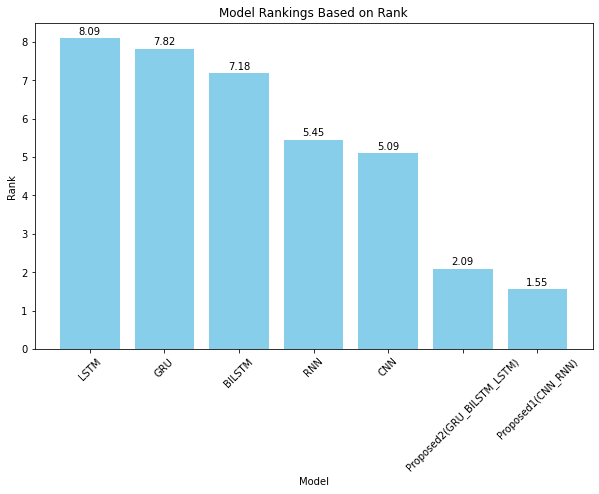
\includegraphics[width=\textwidth]{friedman ranking}
\caption{Friedman ranking of proposed models and traditional DL models}
\label{Line plot12}
\end{figure*}







\section{Conclusions and Future work}
In this work, we studied alternate models for solar irradiance forecasts over various geographic regions. The RMSE was employed as a performance parameter to evaluate each model's accuracy. Models such as RNN, BiLSTM, LSTM, GRU, and CNN were investigated, as well as two suggested hybrid models, "Proposed1 (CNN-RNN)" and "Proposed2 (GRU-BiLSTM-LSTM)." The results reveal that model performance varies by location. Notably, in terms of performance, the suggested hybrid models outperform classic deep learning models. The following are the RMSE values for each location:
The GRU model has the lowest RMSE in Udaipur. The RMSE values in New Delhi vary among models, with LSTM and GRU performing best. Bhuj fared equally across models, with the lowest RMSE coming from the BILSTM model. Across all models, Bengaluru had the highest RMSE values, showing that estimating irradiance in this area is difficult. The model's performance varied in Hyderabad, Ahmedabad, Ahmedabad2, Pokhran, South Delhi, Ajmer, and Jodhpur, demonstrating the impact of local climatic conditions.
The forecasting model should be chosen considering the specific geographical area and meteorological factors. The suggested hybrid models, "Proposed1 (CNN-RNN)" and "Proposed2 (GRU-BiLSTM-LSTM)," have the potential to increase the accuracy of estimations of solar irradiation. Additional study and development of these models may increase their application in renewable energy management systems. This research illuminates the topic of solar energy forecasting, allowing for better-informed decisions on renewable energy integration and resource management.






% \begin{itemize}
%\item
%\item

%\end{itemize}


\section*{CRediT authorship contribution statement}
\textbf{Amod Kumar:} Conceptualization, Methodology, Software. \textbf{Amod Kumar:} Data curation, Writing- Original draft preparation. \textbf{Amod Kumar:} Visualization, Investigation. \textbf{Vipin kumar:} Supervision. \textbf{Amod Kumar:} Software, Validation. \textbf{Amod Kumar and Vipin Kumar:} Writing- Reviewing and Editing.
\section*{Data availability}
The NASA POWER (Prediction of Worldwide Energy Resources) Data Access Viewer website is a massive and open-access library of meteorological, climatological, and renewable energy-related data that may be used by academics, scientists, and professionals all around the globe. The website, which has global geographic coverage, provides a wide range of information on periods ranging from hourly to monthly, including temperature, precipitation, wind speed, solar radiation, insolation, and more. Notably, it satisfies the needs of a wide range of research disciplines by distributing data in several formats and offering user-friendly interactive tools for data manipulation and visualisation. Its open access policy promotes transparency and cooperation, making it a dependable resource for climate studies, renewable energy appraisal, environmental research, and other purposes.

%\section*{Acknowledgments}
\label{}

% Numbered list
% Use the style of numbering in square brackets.
% If nothing is used, the default style will be taken.
%\begin{enumerate}[a)%\item
%\item
%\item
%\end{enumerate}

% Unnumbered list
%\begin{itemize}
%\item
%\item
%\item
%\end{itemize}

% Description list
%\begin{description}
%\item[]
%\item[]
%\item[]
%\end{description}


\begin{comment}

\begin{table}[<options>]
\caption{}\label{tbl1}
\begin{tabular*}{\tblwidth}{@{}LL@{}}
\toprule
& \\ % Table header row
\midrule
& \\
& \\
& \\
& \\
\bottomrule
\end{tabular*}
\end{table}



\end{comment}
% Uncomment and use as the case may be
%\begin{theorem}
%\end{theorem}

% Uncomment and use as the case may be
%\begin{lemma}
%\end{lemma}

%% The Appendices part is started with the command \appendix;
%% appendix sections are then done as normal sections
%% \appendix




\label{}

% To print the credit authorship contribution details
\printcredits

%% Loading bibliography style file
%\bibliographystyle{model1-num-names}
\bibliographystyle{cas-model2-names}

% Loading bibliography database
\bibliography{ref}

% Biography
\bio{}
% Here are the biography details.
\endbio

%\bio{pic1}
% Here are the biography details.
\endbio

\end{document}

